\documentclass[twocolumn,10pt]{article}

%%%%%%%%%%%% PACKAGES %%%%%%%%%%%%%%%%%%%%%%%%%%%%%%%%%%%%%%%%%%%%%%%%%%%%%%%%%%

\usepackage[pdftex]{graphicx}
\usepackage{cite}
\usepackage[cmex10]{amsmath}
\usepackage[sf,sl,outermarks]{titlesec}
\usepackage{caption}
\usepackage{mathptmx}
\usepackage{titling}
\usepackage{tabularx}
\usepackage[utf8]{inputenc}
% \usepackage{tikz, pgf, tkz-euclide}

%%%%%%%%%%% STYLE SETTINGS %%%%%%%%%%%%%%%%%%%%%%%%%%%%%%%%%%%%%%%%%%%%%%%%%%%%%

% \usetikzlibrary{calc, arrows, shapes}
% \usetkzobj{angles} % important you want to use angles

% \graphicspath{../graphics}
% \DeclareGraphicsExtensions{.pdf,.jpeg,.png}

\hyphenation{op-tical net-works semi-conduc-tor}
\bibliographystyle{IEEEtran}

%% section title formatting
\titleformat{\section}  {\bfseries\MakeUppercase}{\thesection}{1em}{}
\titlespacing{\section}  {0pt}{\baselineskip}{0pt}
%% subsection title formatting
\titleformat{\subsection}  {\it\normalsize}{\thesubsection}{1em}{}
\titlespacing{\subsection}  {0pt}{0pt}{-5pt}

\pagenumbering{gobble} % turn off page numbering

%% font stuff
\renewcommand{\rmdefault}{ptm}
% caption
\captionsetup[figure]{labelfont={small},textfont={it,footnotesize},format={hang}}
\captionsetup[table]{labelfont={small},textfont={it,footnotesize},format={hang}}

\interdisplaylinepenalty=5000

%% geometry stuff %%
\setlength{\droptitle}{-.6in} % title position
\setlength{\textheight}{9.25in}
\setlength{\columnsep}{2.0pc}
\setlength{\textwidth}{6.8in}
\setlength{\topmargin}{0.25in}
\setlength{\headheight}{0.0in}
\setlength{\headsep}{-0.4in}
\setlength{\oddsidemargin}{-.19in}
\setlength{\parindent}{0pc}
\setlength{\parskip}{\baselineskip}

%%%%%%%%% DOCUMENT BEGINNING %%%%%%%%%%%%%%%%%%%%%%%%%%%%%%%%%%%%%%%%%%%%%%%%%%%

\begin{document}

%%%%%%%%%%%%%%%%%
%% Top Matters %%
%%%%%%%%%%%%%%%%%

\title{\textbf{An On-Line Visual Driver Aid for Safe and Precise Convoy Following in Visibility-Impaired Conditions}}
\author{
  Robert Cofield, Scott Martin and David Bevly \\
  \em{GPS \& Vehicle Dynamics Laboratory (GAVLab)} \\
  \em{Auburn University} \\
  % Email: robertgcofield@auburn.edu
}
\date{} %% kill date
\maketitle

%%%%%%%%%%%%%%
%% Abstract %%
%%%%%%%%%%%%%%

\begin{abstract}

  % good intro of what is being presented.
  A graphical driver aid based upon GNSS positioning is presented which will augment or replace visual cues in scenarios where line-of-sight is unreliable or unavailable, regardless of the ground-based deployment platform.
  % positioning algorithms used
  Dynamic-base Real-Time Kinematic (DRTK) GPS is used to find a relative position from the leader to the follower, while the Time Differenced Carrier Phase (TDCP) measurement is used to compute the change in position of both vehicles over time.
  % relative path vectorization
  The relative path vector method proposed by \cite{travisdiss} is used to compute the positions of a virtual leader, i.e., a series of points representing where the leader was at previous time steps.
  % GUIs
  This path is then displayed to following drivers using two graphical user interfaces (GUIs): a minimalistic design relaying only necessary information, and a design incorporating satellite imagery to give the driver information to localize the displayed path.
  % testing
  The effectiveness of these tools is then evaluated by recording and analyzing the path following performance in various scenarios.

\end{abstract}

%%%%%%%%%%%%%%%
%% Biography %%
%%%%%%%%%%%%%%%

\section*{Biography}

  Robert Cofield is investigating navigation of ground and other vehicles using GNSS and fused sensor solutions.  He works in the Auburn University GPS \& Vehicle Dynamics Laboratory.

%%%%%%%%%%%%%%%%%%%%%%%%%%%%%%%%%%%%%%%%%%%%%%%%
%% Introduction %% Previous Work & Literature %%
%%%%%%%%%%%%%%%%%%%%%%%%%%%%%%%%%%%%%%%%%%%%%%%%

\section*{Introduction}

  %%%%% Intro Blurb - why important %%%%%
  The use of vehicle convoys is commonly used in ground transportation, and both safety and path precision are often of chief importance to this task.  Extremely close spacing can be used to reduce fuel costs, but introduces a collision risk.  In other cases, when traveling over a path that has unstable or dangerous areas nearby, a following vehicle attempts to stay within the track of a vehicle ahead.  When visibility is impaired, the ability of any convoy driver to adhere to a path of known safety and to avoid colliding with the leader is significantly reduced.  Real-time path information is sought which will enable a following driver to intuitively and safely maintain a high-fidelity execution of the desired path during situations in which the leader is either not directly visible or close enough that the risk of collision is imminent.

  % Problem specific - why two vehicles were used
  For the convoy scenario, a caravan of $N$ vehicles attempting to travel along the same path may be broken down into $N-1$ leader-follower pairs.  These pairs may comprise each of the longitudinally adjacent vehicles.  Alternatively, the convoy leader may be the leader for each pair, where the follower is each of the other vehicles in the conoy.  For the development of a path following driver aid, however, the configuration was simplified to a single pair of vehicles.  It was assumed that a single stream raw range and carrier measurements would be received from the vehicle whose path should be replicated.


%%%%%%%%%%%%%%%%%%%%%%%%%%%%%%%%%%%%%%
%%%%% Literature & Previous Work %%%%%
%%%%%%%%%%%%%%%%%%%%%%%%%%%%%%%%%%%%%%

\section*{Previous Work}
  % scott and will
  % General situational awareness
  Situational awareness systems (SASs) ... 
  % sandia situational awareness
  Researchers at Sandia Laboratories \cite{riblett2007} developed a vehicular situational awareness system based upon ad-hoc communications, which utilizes a touch-screen display of other vehicles. This system was then extended to operate in dismounted situations via a handheld display device.
  %%!! Blue force tracker
  %%! Robotic path following
  % Path information display is not common
  The literature has very few examples of SASs which track and relay relative path information. This work seeks to explore that area further and provide a novel solution to the human-controlled path following problem.\

  This work follows and builds upon that done by Martin \cite{ScottThesis} and Travis \cite{travisdiss}.
  % DRTK
  DRTK is a feature now common on many GPS receivers, with \textbf{Finish}
  
  The driver aid presented herein extends the DRTK/TDCP following algorithm by combining relative path data with standard GPS estimates for velocity and course as shown in Fig. \ref{fig:data_flow} below.

  %% Input from GPS / DRTK / TDCP
  \begin{figure}[ht] \centering
    \includegraphics[width=0.8\columnwidth]{../graphics/data_algo.png}
    \caption{Data flow from GNSS receivers to the GUI backend}
    \label{fig:data_flow}
  \end{figure}


%%%%%%%%%%%%%%%%%
%% GUI Display %%
%%%%%%%%%%%%%%%%%

\section*{Graphical User Interface}

  % Overarching design goals
  From the outset, a primary design goal was to minimize the amount of visual and cognitive effort required on the part of the driver in determining whether course and speed corrections are necessary, and if so, what they are.

  %% Alerts
  Apart from relaying the relative path and leader's velocity and course, two other pieces of information need to be determined: separation between the two vehicles, and by how much the following vehicle strays from the desired path.
  % define lateral deviation
  Lateral deviation is measured by the magnitude of a line passing through the position of the follower and perpendicularly intersecting the nearest path segment.
  % define path distance
  Curvilinear path separation is defined as the summed distance along the computed relative path from the leader (the last point in the path) to the point where the lateral deviation line intersects the path.

  % \begin{figure}[ht] \centering
  %   \scalebox{.8} {\input{../graphics/devpts_diagram}}
  %   \caption{Points used for deviation calculation}
  %   \label{fig:pathpts}
  % \end{figure}

  %% User input parameters relating to alerts
  To determine whether these values are acceptable, thresholding was implemented to differentiate between three possible states, deemed `acceptable', `warning', and `critical'.
  For lateral deviation, these values are as simple as 
  % 
  Facilities for accepting these driver-input operational parameters must therefore be obscured during the driving task, yet easily accessible on the fly. 

  \textbf{Course Spinning}

  %% Qt %%
  \subsection*{Qt}
  
    % overall reasoning for the Qt GUI 
    A clean and minimal visual presence ensures that a passing glance is sufficient to check on distance and deviations.  When following very closely, a follower will need to anticipate upcoming turns without being able to see the leader actually turn, so course information---specifically, the leader's course relative to that of the follower---will be needed.  These were the fundamentals driving the GUI development at the outset.  The resulting interface was presented in a single window on the display device and utilized only the Qt4 C++ library \cite{qt} and associated Python bindings for rendering.

    \begin{figure}[ht] \centering
      \includegraphics[width=\columnwidth] {../graphics/final_design_data.png}
      \caption{Qt GUI in normal operation}
      \label{fig:qt_normal}
    \end{figure}

    %% Display explanation
    % follower-forward is up on the screen
    All information is displayed such the `up' on the display device corresponds to the positive longitudinal axis of the following vehicle.
    % orientation of path and leader is determined using the follower course
    Since the relative path is computed in ECEF coordinates and converted into relative ENU components, displaying points of interest relative to the follower's orientation is done by rotating them using the course measurement of the following vehicle's receiver. For low-dynamic scenarios, approximating heading as being equivalent to course provided adequate results.
    % orientation of leader course
    The orientation of the lead vehicle (represented with a simple square icon containing an arrow for its positive longitudinal axis) is then always shown relative to the follwing vehicle.  So if the leader is shown pointing to the right, the direction of its motion is then to the follower’s lateral axis and in the positive direction. 


  %% Earth %%
  \subsection*{Google Earth}

    % motivation for using earth
    Since a significant end use case involves military convoys, feedback was sought from personnel in the Armed Forces.  One primary criticism was the lack of visual stimuli by which to reconcile the screen output with what the user sees around them.  In essence, it was suggested, users must develop a trust with any tool before beginning to make decisions based upon it, particularly in the dire situations for which this tool is designed.  To remedy this, it was proposed that satellite imagery be incorporated into the background of the information already displayed on the screen.  As this directly contradicted the clean, distraction-free nature of the prototype already developed, it was determined that another version needed to be constructed following these new design principals, and that the two GUI's should be juxtaposed the most prudent approach.  In determining what software package to use as an imagery backend, a trade study was performed and the resulting candidates were narrowed to Quantum GIS and Earth (by Google).  The maturity, user-base and documentation on representing data with the Keyhole Markup Language (KML) ultimately made Google Earth the favored tool.

    \begin{figure}[ht] \centering
      \includegraphics[width=\columnwidth] {../graphics/earth_slow.png}
      \caption{Google Earth GUI alerting user to slow and correct leftward}
      \label{fig:earth_alerts}
    \end{figure}

    % note about adding leader velocity
    % placement by follower std position
    Switching to Google Earth necessitated provided at least one global position by which to overlay all the data relative to the follower.  The standard positioning solution for the follower is used for this, meaning that all positions as they are displayed have centimeter-level relative accuracy, but accuracy relative to the underlying satellite imagery is contingent upon both the receiver used and the accuracy of the satellite images.  As the accuracy of Google Earth imagery varies with location, and can be off by as much as 50 m \cite{ge_accuracy}, improving the global accuracy was determined to be of low importance.  As 
    % path and leader orientation implicit since path is in E,N coordinates

  %% Interpolator Section %%
  \subsection*{Live Interpolation}

    % had to interpolate to smooth
    The addition of satellite imagery made the user highly aware of the update rate of each piece of information displayed spatially, as the terrain view was refocused on each update.  This necessitated the incorporation of data smoothing techniques to prevent the user from becoming disoriented.
    % linear interpolation - lag
    Since the primary object is to display information that has been received rather than predict future states, a minimum of two of the most recent data points is required to do a live interpolation.  With this, a continuous-time linear interpolation of the measurement at any instant between those two times is possible.  By making more data points available and considering the type or nature of data in question, more accurate forms of interpolation may be possible. However, due to speed and efficiency concerns, the linear interpolation is preferable in this situation.
    % interpolation vs synchromization
    A simpler approach to reducing the number of updates is to synchronizing all data using GPS timestamps by holding asynchronous packets until all data packets have been received.
    
    All values which are displayed in the GUI are passed through the interpolation algorithm when this smoothing mode is enabled.
    For two dimensional positions, this procedure is carried out on both the East and North coordinates. 
    %% path
    For the path to be interpolated,  the same procedure for positions is carried out for each point in the vector. A problem arises when interpolating between timesteps with unequal numbers of points, as each point cannot then be interpolated as if it were travelling along a line. When path length mismatch occurs between two successive updates, redundant points are added coincident with the rearmost path point until the two vectors are equal in length. When the number of points is decreasing, this alone would lead to a buildup of unnecessary data points, tying up valuable memory space and processing time. Thus, each time the length decreases and stays constant or continues decreasing for two or more timesteps, redundant points are removed from the saved vector.

    \begin{figure}[ht] \centering
      \includegraphics[width=\columnwidth]{../graphics/middleware_diagram.png}
      \caption{Delivery of data from the middleware interface to the GUI backend}
      \label{fig:middlewared}
    \end{figure}

    %% time update
    While GNSS provides the ability to precisely synchronize systems, display smoothing must rely upon computer-specific timestamps as some machines will operate more slowly than others. Accordingly, when initial measurement messages arrive, the CPU time at which the content of each message packet was extracted is stored along with that content. It is important that CPU time is recorded upon extraction rather than upon completion of processing or transmission, as the goal of this process is to obscure lags incurred during calculation or radio transmission; the extraction (and assignment) time represents the earliest point when any portion of the rest of the GUI may then access that data to display it. The end result is that the user is presented with data which will change at a consistent frequency (as specified by the user), regardless of whether multiple sensors take varying amounts of time to relay or calculate data.

    %% REDO THIS WITHOUT EQUATION STUFF
    % Upon each subsequent measurement update, the two previously newest values $(x_1,t_1)$ are moved to variables for old data $(x_0, t_0)$ and the new value is stored along with present CPU time. An interpolation object representing Eq. \eqref{eq:interp} is created with the present data so that between times $t_0$ and $t_1$ an input $t$ will yield the respective measurement $x$. Any interpolation thread which is still running is then stopped, and a new one spawned. This thread begins incrementally calculating data between $x_0$ and $x_1$, then waits a period of time corresponding to the desired frequency, repeating until either a new measurement update occurs or time $t_1$ is reached.


%%%%%%%%%%%%%%%%%%%%%%%%%%%%%%%%%%%%%%%%%%
%% Experimentation Procedures & Results %%
%%%%%%%%%%%%%%%%%%%%%%%%%%%%%%%%%%%%%%%%%%

\section*{Experimentation}

  Experimental trials were conducted using three different testing scenarios: the lane-change test, the precision following test, and the zero landmark test.  
  %% Hardware
  The GNSS hardware used were both L1/L2 NovAtel Propak v3 (using OEMV chips). The DRTK and TDCP estimators utilized both L1 and L2 signals, from GPS satellites only.  Raw pseudorange and carrier information was broadcast directly from the lead receiver to the navigation computer in the following vehicle using two 900 MHz radios. To prevent the length of the vehicles from introducing constant biases into the estimate of longitudinal curvilinear spacing, the lead vehicle's antenna was placed on the most rearward horizontal surface and the following vehicle's antenna was placed on the most forward horizontal surface.
  % display
  A single laptop computer was used for the differential GPS calculations as well as the display control. This was placed in the following vehicle in direct view of the driver, as shown in Figure \ref{fig:driver_view}.

  \begin{figure}[ht] \centering
    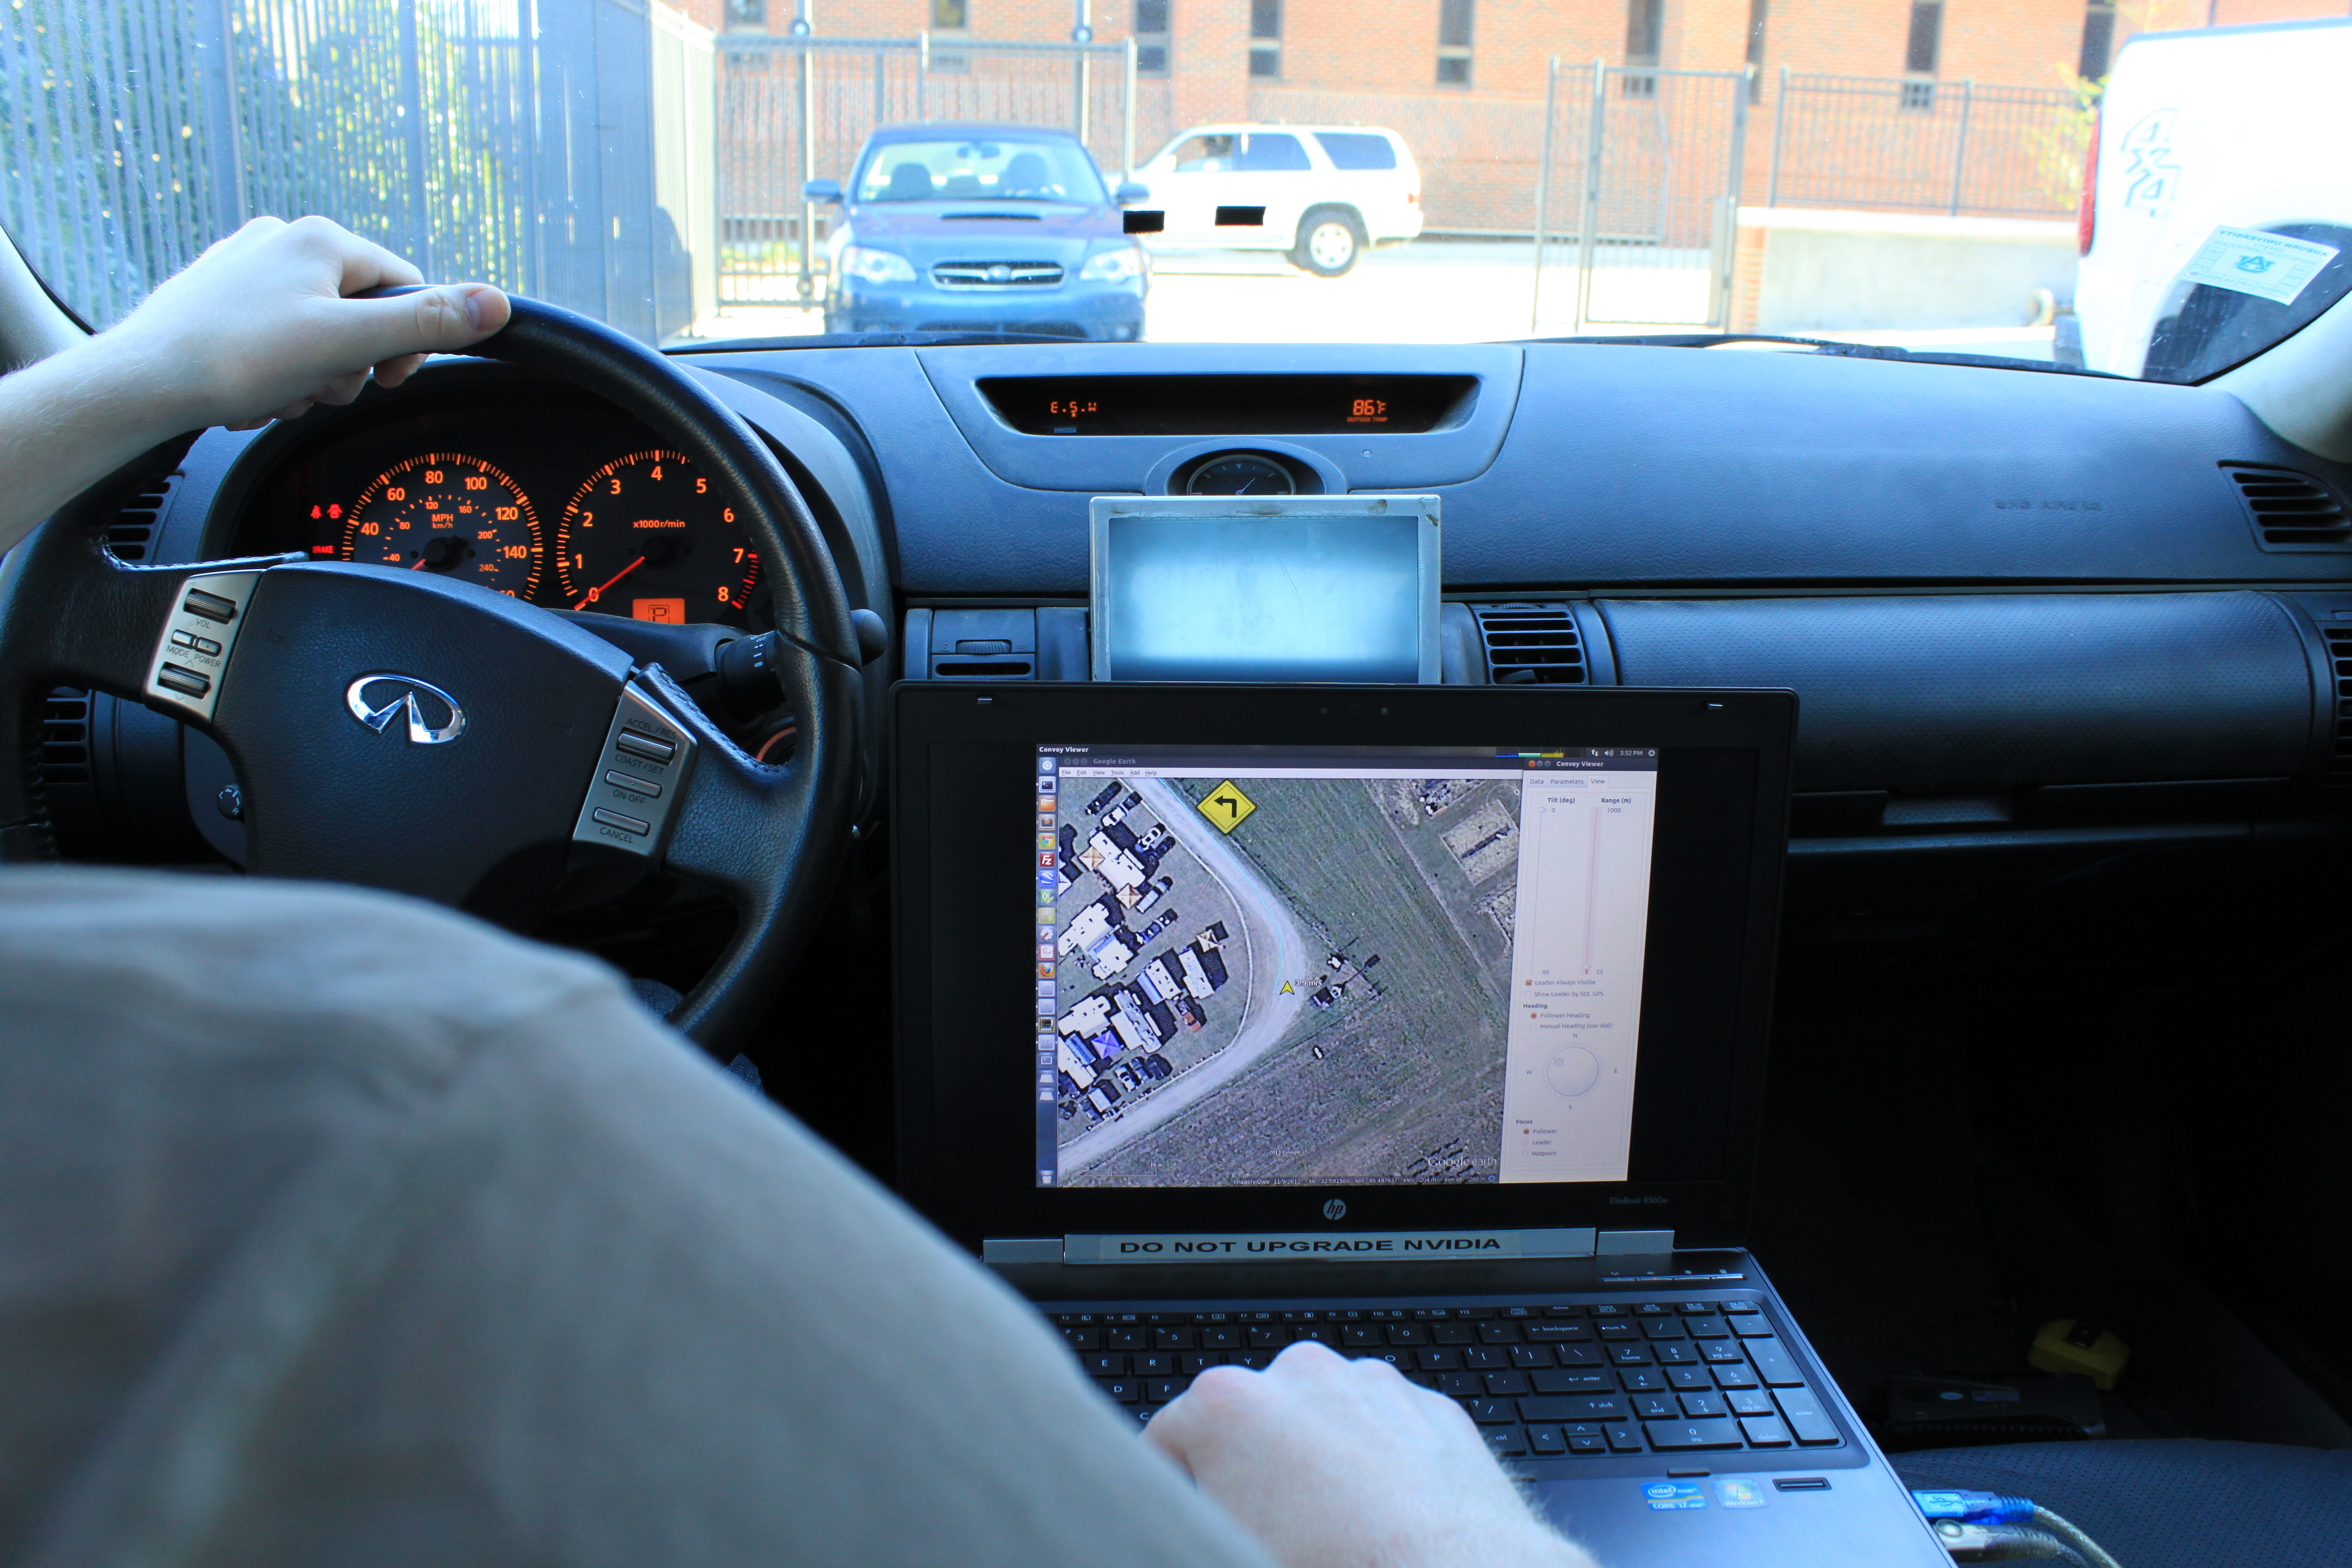
\includegraphics[width=0.8\columnwidth]{../graphics/driver_view.jpg}
    \caption{The display computer was placed in direct view of the following driver.}
    \label{fig:driver_view}
  \end{figure}

  For all tests, the same set of alert thresholds were used to ensure consistency. A lateral deviation warning alert was issued at 1.0 m, and a lateral deviation critical alert was issued at 2.0 m. A longitudinal spacing warning alert was issued at $\mu = 0.5$ and a longitudinal spacing critical alert was issued at $\mu=1.0$.
  \textbf{TODO Default threshold determination}

  % Results analysis:
  For both the precision following and zero landmark tests, the combined percentage of timesteps in which either a deviation or distance alert was present was calculated to find the `best' run of that test, one for each of the GUIs, and one without any aid (the control). These data runs are then analyzed in depth below.

  %% Lane-Change Test
  \subsection*{Lane Change Test}

    % explanation of test
    To produce pass-fail results, a maneuver common in typical roadway driving, the lane change, was used in a situation in which the maneuver could be replicated properly or improperly to produce a binary result.  This test takes place on the National Center for Asphalt Technology (NCAT) test track in Opelika, AL, which is a two lane, 1.7 mile oval with turns comparable to those found on an interstate highway.  The leader drives through a $180^{\circ}$ turn and upon exiting makes a lane change between any of six cones spaced $10~m$ apart along the center stripe at the start of the straightaway.  This event is visually obscured from the following driver, who has no foreknowledge of which cone pair will be chosen, so there is a 20\% chance of choosing the correct pair simply by guessing.

    \begin{table}[htbp] \centering
      \caption{Cone pairs chosen in the lane change replication test}
      \begin{tabular}{rc|cc} 
        GUI&    Run \#  &     Leader&    Follower \\\hline\hline
        Earth&      1       &       1   &    3 \\
             &      2       &       3   &    4 \\ \hline
        Qt   &      3       &       2   &    3 \\
             &      4       &       5   &    5 \\ \hline   
      \end{tabular}
      \label{tab:lanechangeresults}
    \end{table}



  %% Precision Following Test %%
  \subsection*{Precision Following Test}

    % motivation
    The lane change replication test is one example of implementing the path duplication tool, but does not produce the detailed results necessary for a formal conclusion favoring the usefulness of one GUI over the other.  Centimeter-level measurements are available, so it is of great interest to determine whether either tool enables a convoy driver to carry out the following task with this improved level of precision.
    
    % description
    The precision following test begins and ends with both vehicles parked atop the center stripe of the NCAT test track.  The lead vehicle accelerates to approximately 45 mph then begins a sinusoidal path with a mean about the center stripe, a period of approximately $10~s$, and an amplitude that puts the wheels of the lead vehicle upon the outermost lane marking at the peaks.  Once reaching 45 mph, the magnitude of the leader’s ground plane velocity vector will vary according to position on the track.  Along the two $180^{\circ}$ turns it will be approximately 45 mph, and along the straightaways it will be approximately 65 mph.  Throughout the test, the following driver is attempting to maintain a inter-vehicular spacing as low as possible without incurring any distance alerts, and accumulate as little deviation over time as possible.

    \begin{figure}[ht] \centering
      \includegraphics[width=\columnwidth]{../graphics/precision_following_alert_percents.png}
      \caption{Percentages of best runs from the precision following test in which alerts were incurred}
      \label{fig:precision_following_alert_percents}
    \end{figure}

    % discussion of the merits of the test
    This test primarily focused on distinguishing which GUI best provided aid in path duplication; for a comparative analysis, the test was conducted with the aid of each GUI individually, then without any assistance information at all.  As this test was conducted in an environment equivalent to most American two-lane roads and the leader does not stray from the two outer lane markings, it was anticipated that the lateral deviation should be bounded by approximately the width of the road minus the track width of the widest vehicle, or $5.8~m$.  This allows for scrutiny of the deviation in greater detail than when the lateral deviation is not bounded by design.

    %% discussion of Results



  %% Zero-Landmark Test %%
  \subsection*{Zero-Landmark Test}

    % motivation
    The precision following test took place in an environment abundant in visual landmarks by which to localize, such as lane markings and road signs.  Given the motivation for these tools, it is necessary to examine the performance of both GUIs in a situation where this type of assistance is denied.  The zero landmark test was therefore constructed to determine the impact of removing visual awareness of surrounds as well as waypoints along the leaders path to assist in replicating it.
    
    \begin{figure}[ht] \centering
      \includegraphics[width=\columnwidth]{../graphics/zero_landmark_alert_percents.png}
      \caption{Percentages of best runs from the zero landmark test in which alerts were incurred}
      \label{fig:zero_landmark_alert_percents}
    \end{figure}

    % test description
    Both vehicles began parked in a large, open expanse of flat asphalt (`skidpad') with excellent satellite visibility.  There are no clearly visible artifacts upon the ground, though some objects are visible at the outer edges of the skidpad.  To further obscure visual following, the test was conducted at night.  The lead vehicle drove in chaotic patterns intended present a path with is difficult to follow while the following vehicle attempted to adhere to the path as well as possible and maintain the closest possible curvilinear separation distance without triggering any alert messages.

    % discussion of results

  %% Deviation for PF and ZL tests %%
  \begin{table}[htbp] \centering
    \caption{Mean absolute deviation for the precision following \& zero landmark tests}
    \begin{tabular}{r|c|c|} 
      GUI&         Precision Following & Zero Landmark \\
      \hline
      Earth&      0.9677 m & 2.7404 m \\
      Qt&         0.4719 m & 3.6830 m \\
      Control&    0.2069 m & 0.7267 m \\ \hline 
    \end{tabular}
    \label{tab:zero_dev_mean}
  \end{table}


%%%%%%%%%%%%%%%%%%%%%%%%%%%%%%%
%% Conclusions / Future Work %%
%%%%%%%%%%%%%%%%%%%%%%%%%%%%%%%

\section*{Conclusions \& Future Work}

  %% summary
  Two graphical tools were developed to assist drivers in convoys with high fidelity to the lead vehicle’s path while maintaining a safe spacing between them.  Experimentation reveals that they were quite effective in helping to enforce safe curvilinear following distances, while more development is needed to optimize results for lateral path deviation.  

  %% improvements - overlay prediction
  The zero landmark test was by far the most successful in garnering qualitative feedback.  Drivers suggested a projected path overlay which gave a prediction of the follower’s path in realtime given course and yaw rate information.  This would counter the effects of being unable to tell how present actions would effect deviation in the approximately 1 s required for steering input to be reflected in either GUI.  Furthermore, it was suggested, a model prediction scheme as in \cite{williamthesis} could be employed to show not only predicted path over some window, but estimate the current position and overlay it.  Future work will pursue adding these improvements to the Qt GUI and continuing to refine that tool, as it has been shown more successful than the Earth GUI at accomplished the goals outlined herein.

  %% add SA for the whole caravan - Yuma
  %% magnetometry for course/heading


%%%%%%%%%%%%%%%%%%%%%%%%
%%%%% Bibliography %%%%%
%%%%%%%%%%%%%%%%%%%%%%%%

\nocite{CofieldUGThesis}
\bibliography{../bib/master}


\end{document}